\documentclass{article}

\usepackage{amsmath}
\usepackage{amssymb}
\usepackage{hyperref}
\usepackage{indentfirst}
\usepackage{listings}
\usepackage{xcolor}
\usepackage{graphicx}
\lstset{language=C++,
                basicstyle=\ttfamily,
                keywordstyle=\color{blue}\ttfamily,
                stringstyle=\color{red}\ttfamily,
                commentstyle=\color{green}\ttfamily,
                morecomment=[l][\color{magenta}]{\#}
}

%User defined commands
\newcommand{\sgn}{\operatorname{sgn}}

\begin{document}
\begin{center}
	\huge{\bf CSE 120: Homework 2} \\
	Merrick Qiu
\end{center}

\begin{enumerate}
    \item \begin{lstlisting}
struct lock {
    bool* flag = false;
}

void acquire (struct lock *) {
    bool lockedFlag = true;
    while (true) {
        if (lock == 0) {
            XCHG(lockedFlag, lock->flag);
            break;
        }
    }
}

void release (struct lock *) {
    (lock->flag)* = false;
}
   \end{lstlisting}
    \item \begin{enumerate}
        \item main, A, B, A
        \item fee foe foo far fie fum fun
        \item The currentThread will be main and 
        the ready and wait queues will be empty.
    \end{enumerate}
\item \begin{enumerate}
\item \begin{lstlisting}
monitor Barrier {
    int doneThreads = 0;
    Condition barrier = new Condition();

    void Done(int n) {
        doneThreads++;
        if (doneThreads = n) {
            doneThreads = 0;
            barrier.wakeAll();
        } else {
            barrier.wait();
        }
    }
}
\end{lstlisting}

\item \begin{lstlisting}
class Barrier {
    int doneThreads = 0;
    Lock lock = new Lock();
    Condition barrier = new Condition();

    void Done(int n) {
        acquire(lock);
        doneThreads++;
        if (doneThreads = n) {
            doneThreads = 0;
            barrier.wakeAll();
        } else {
            barrier.wait();
        }
        release(lock);
    }
}
\end{lstlisting}
    \end{enumerate}
    \item 
\begin{lstlisting}
class Surfing {
    enum State { calm, breaking; }
    enum Direction { LEFT, RIGHT, BOTH; }

    State oceanState = calm;
    Direction waveDirection = BOTH;
    Condition leftDirection = new Condition();
    Condition rightDirection = new Condition();
    Lock lock = new Lock();

    void paddle (Direction dir) { // invoked by surfer threads
        acquire(lock);
        if (oceanState == breaking && waveDirection == dir OR BOTH) {
            // successful paddle
            release(lock);
            return;
        }
        (dir == left ? leftDirection : rightDirection).wait();
        release(lock);
    }
    void wave (Direction dir) {   // invoked by the ocean thread
        acquire(lock);   
        oceanState = breaking;
        waveDirection = dir;
        if (dir == left OR BOTH) {
            left.wakeAll();
        } 
        if (dir == right OR BOTH) {
            right.wakeAll();
        } 
        release(lock);
    }
    void done () {                // invoked by the ocean thread
        acquire(lock);
        oceanState = calm;
        release(lock);
    }
\end{lstlisting}
\item 
From the diagram, we can see that having the students work in the order of 
Bertrand, Dag, Chloe, then Annabelle 
lets everyone get their work done.
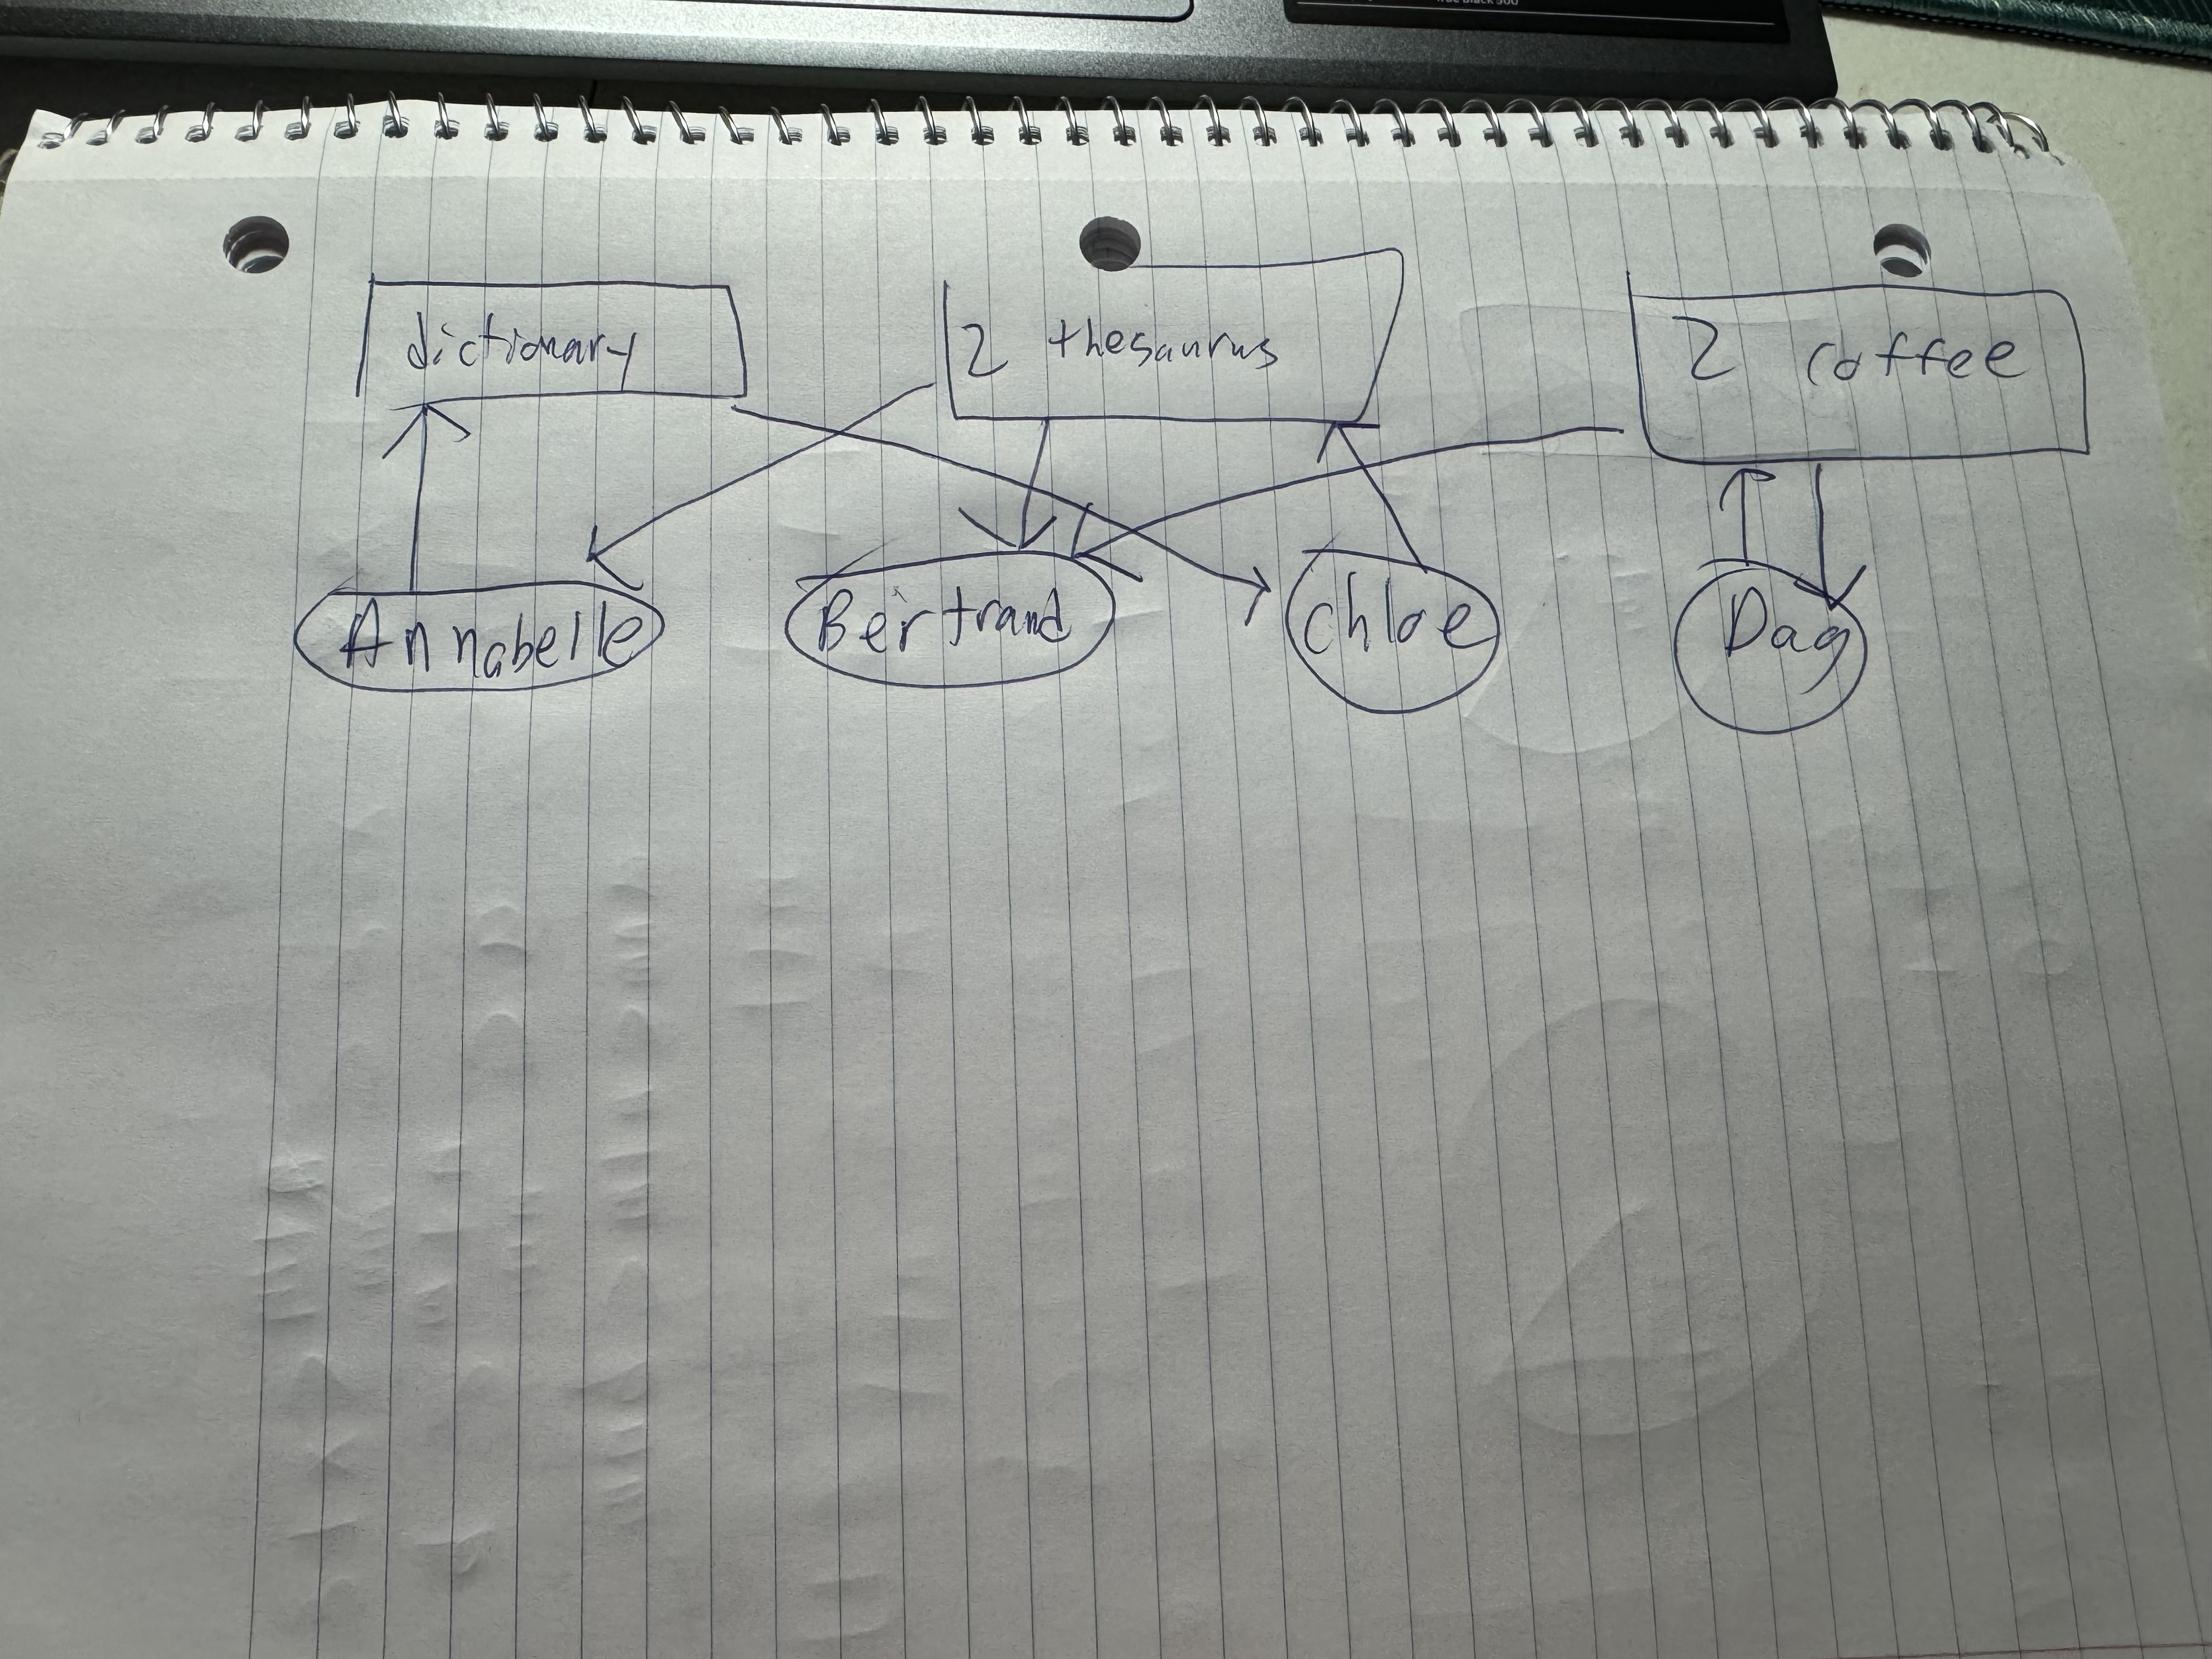
\includegraphics[width = 15cm]{diagram.jpg}

\end{enumerate}




\end{document}